\documentclass[xcolor=table, aspectratio=169, bigger]{beamer}

\usepackage{shyne}

% Theme settings
\setbeamertemplate{navigation symbols}{}

\usetheme{Madrid}
\usefonttheme{structurebold}
\usefonttheme[onlymath]{serif}

\AtBeginSection[]
{ 	\begin{frame}{}

	{
	\usebeamerfont{frametitle}
	\begin{beamercolorbox}
		[wd={\textwidth}, center, sep=.2in, rounded=true, shadow=true]
		{frametitle}
	Week \thesection\\  \secname 
	\end{beamercolorbox}
	}
	
	\end{frame} 
}

\AtBeginSubsection[]
{ 	\begin{frame}{}

	{
	\usebeamerfont{frametitle}
	\begin{beamercolorbox}
		[wd={\textwidth}, center, sep=.2in, rounded=true, shadow=true]
		{frametitle}
	Section \thesection .\thesubsection\\  \subsecname 
	\end{beamercolorbox}
	}
	
	\end{frame} 
}

\title[Week 4]{Stat 201: Statistics I\\ Week 4 }
\author[M. Shyne]{}
\institute[Metro State]{
\includegraphics[width=1.75in]{../images/metro_logo}}
\date[2/10/2019]{
\\ \bigskip \bigskip 
\includegraphics[width=.4in]{../images/cc_big}}



\begin{document}
\frame{\titlepage}

%
% Week 4
%
\setcounter{section}{3}
\section{Examining and Summarizing Data}

%
% Section 4.1
%
\subsection{Summarizing and Plotting Data Distributions}

%%%%%%%%%%
\begin{frame}
\frametitle{Frequency distributions}

\begin{block}{}
A \bt{frequency} is the number of times a particular value occurs in a set of data, i.e. the count.
\end{block}
\pause
\begin{block}{}
A \bt{frequency distribution} (or \bt{frequency table}) summarizes a set of data by listing the frequencies of data in categories or classes (groups).
\begin{itemize}
\item For categorical data, the categories are simply the possible values of the data.
\item For quantitative data, the classes are usually ranges of possible values.
\end{itemize}
\end{block}
\end{frame}

%%%%%%%%%%
\begin{frame}
\frametitle{Frequency distribution for categorical data}

\begin{exampleblock}{Example}
\bt{Favorite kind of taco} = \{Chicken, Fish, Fish, Veggie, Chicken, Beef \}
\pause
\begin{center}
\begin{tabular}{c | c}
Kind of taco & Frequency\\
\hline
Beef & 1\\
Chicken & 2\\
Pork & 0\\
Fish & 2\\
Veggie & 1
\end{tabular}
\end{center}
\end{exampleblock}
\end{frame}

%%%%%%%%%%
\begin{frame}
\frametitle{Frequency distribution for quantitative data}

\begin{exampleblock}{Example}
\bt{Tacos eaten} = \{3, 0, 17, 6, 4, 3, 5 \}
\pause
\begin{center}
\begin{tabular}{c | c}
Number of tacos eaten & Frequency\\
\hline
0 - 4 & 4\\
5 - 9 & 2\\
10 - 14 & 0\\
15 -20 & 1
\end{tabular}
\end{center}
\end{exampleblock}
\end{frame}

%%%%%%%%%%
\begin{frame}
\frametitle{Relative frequency}

\begin{block}{}
\bt{Relative frequency} is the proportion (fraction) of the whole data set that resides in each category or class. When expressed as a percent it is called \bt{percentage frequency}.
\end{block}
\pause
\begin{block}{}
To calculate: For each class,
\[\text{Relative frequency} = \frac{\text{class frequency}}{\text{total count}}\]
\[\text{Percentage frequency} = \frac{\text{class frequency}}{\text{total count}} \times 100\]
\end{block}

\end{frame}

%%%%%%%%%%
\begin{frame}
\frametitle{Relative frequency example}

\begin{exampleblock}{Example}

\begin{center}
\begin{tabular}{c | c | c | c}
Tacos eaten & Frequency & Relative & Percentage\\
\hline
0 - 4 & 4 & 0.5714 & 57.14 \%\\
5 - 9 & 2 & 0.2857 & 28.57 \%\\
10 - 14 & 0 & 0 & 0 \%\\
15 -20 & 1 & 0.1428 & 14.28 \%\\
\hline
Total & 7 & 1 & 100 \%
\end{tabular}
\end{center}
\end{exampleblock}

\end{frame}

%%%%%%%%%%
\begin{frame}
\frametitle{Cumulative frequency}

\begin{block}{}
\bt{Cumulative frequency} is the frequency for a class and \emph{all previous classes}.
\end{block}
\pause
\begin{exampleblock}{Example}

\begin{center}
\begin{tabular}{c | c | c }
Tacos eaten & Frequency & Cumulative\\
\hline
0 - 4 & 4 & 4\\
5 - 9 & 2 & 6\\
10 - 14 & 0 & 6\\
15 -20 & 1 & 7\\
\end{tabular}
\end{center}
\end{exampleblock}
\end{frame}

%%%%%%%%%%
\begin{frame}{Histograms}
\begin{block}{}
A \bt{histogram} is a graphical representation of a frequency distribution of quantitative data. This allows the distribution of the data to be more easily visualized.
\end{block}

\pause
\begin{columns}
\begin{column}{0.35\textwidth}
\begin{exampleblock}{}
\begin{center}
\begin{tabular}{cc}
Num tacos & Freq \\
\hline
 $<$ 2 & 10 \\
2 -3 & 27 \\
4 - 5 & 41 \\
6 - 7 & 19 \\
 $\ge$ 8& 3 \\
\end{tabular}
\end{center}
\end{exampleblock}
\end{column}

\begin{column}{0.65\textwidth}
\begin{center}
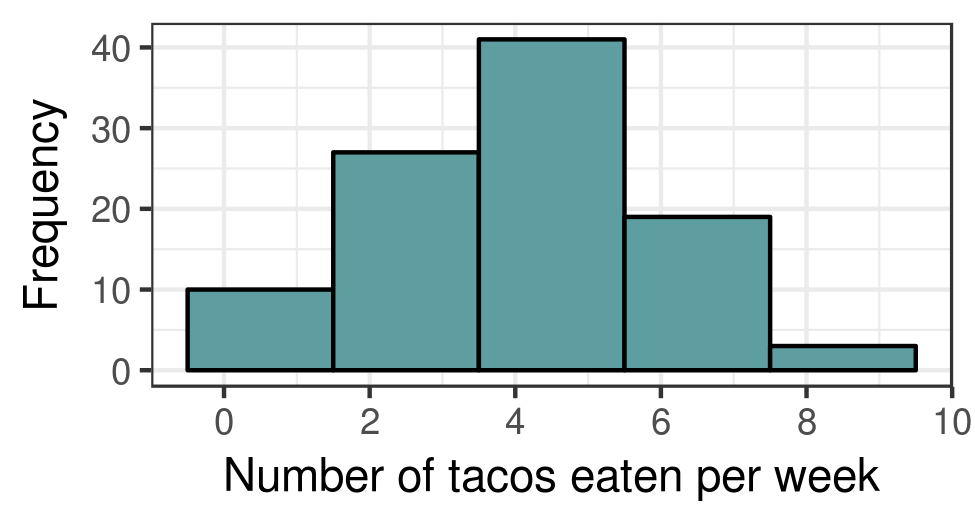
\includegraphics[width=3.25in]{../images/wk04_taco_hist}

\end{center}
\end{column}
\end{columns}

\end{frame}

%%%%%%%%%%
\begin{frame}{Properties of histograms}
\begin{block}{}
\begin{itemize}
\item A graph of bars of equal width drawn adjacent to each other.
\pause
\item The horizontal scale (x-axis) represents values of the quantitative data. Each bar represents a class, or range of values, from a frequency table. 
\pause
\item The vertical scale (y-axis) represents frequency (counts), or proportions (relative frequency) or percentages (percentage frequency).
\pause
\item The number of bars is largely an aesthetic choice. There should be enough bars to adequately show the shape of the distribution, but too many can make a ``busy" graph that's hard to read. Most software will automatically choose the number of bars.
\end{itemize}
\end{block}
\end{frame}

%%%%%%%%%%
\begin{frame}{Outliers}
\begin{block}{}
An \bt{outlier} is a data point that is distant from other data or that deviates from an established pattern.

\begin{itemize}
\item Outliers can result from chance, an unusual subject, or error.
\end{itemize}
\end{block}

\pause

\begin{columns}
\begin{column}{0.35\textwidth}
\begin{exampleblock}{}
\begin{center}
\begin{tabular}{cc}
Num tacos & Freq \\
\hline
 $<$ 2 & 10 \\
2 -3 & 27 \\
4 - 5 & 41 \\
6 - 7 & 19 \\
8 - 9 & 3 \\
10 - 11 & 0 \\
$\ge$ 12 & 1 \\
\end{tabular}
\end{center}
\end{exampleblock}
\end{column}

\begin{column}{0.65\textwidth}
\begin{center}
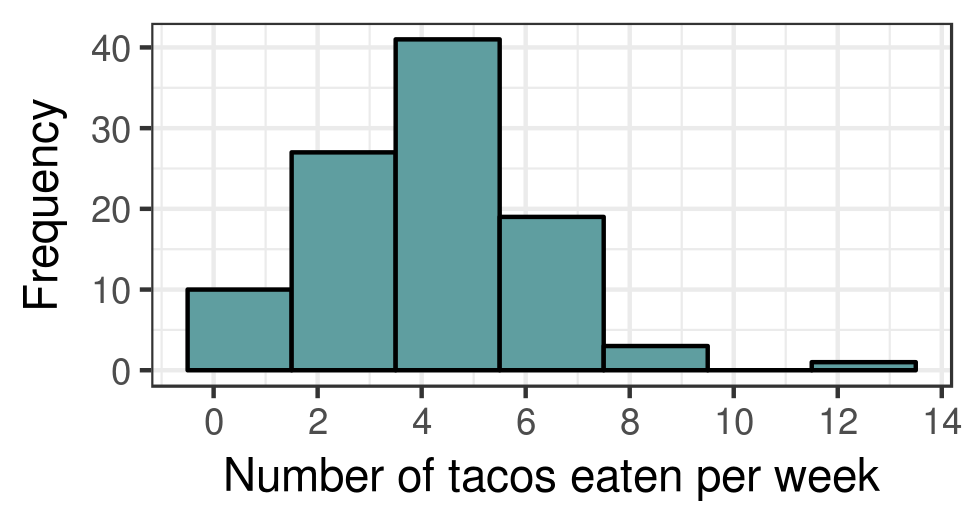
\includegraphics[width=3.25in]{../images/wk04_taco_out_hist}

\end{center}
\end{column}
\end{columns}
\end{frame}

%%%%%%%%%%
\begin{frame}
\frametitle{Normal distributions}

\begin{block}{}
A \bt{normal distribution} can be identified from a frequency table that has the following characteristics:
\begin{itemize}
\item The frequencies start low, increase to a high point and then decrease to low frequencies at the end
\item The frequencies are approximately symmetric around the high point.
\end{itemize}
\end{block}
\end{frame}

%%%%%%%%%%
\begin{frame}{Normal distributions, example}

\begin{columns}
\begin{column}{0.35\textwidth}
\begin{exampleblock}{}
\begin{center}
\begin{tabular}{cc}
IQ & Freq \\
\hline
$<$ 70 & 2 \\
70 - 80 & 24 \\
80 - 90 & 147 \\
90 - 100 & 342 \\
100 - 110 & 339 \\
110 - 120 & 125 \\
120 - 130 & 18 \\
130 - 140 & 3 \\
\end{tabular}
\end{center}
\end{exampleblock}
\end{column}
\pause
\begin{column}{0.65\textwidth}
\begin{center}
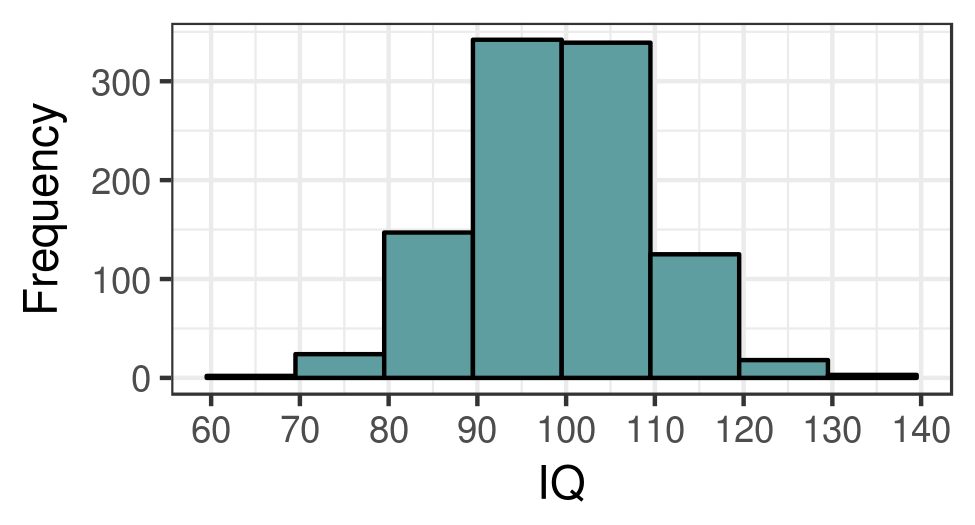
\includegraphics[width=3.25in]{../images/wk04_iq_hist}

\end{center}
\end{column}
\end{columns}

\end{frame}


%%%%%%%%%%
\begin{frame}{Skewed distributions, right skew example}

\begin{columns}
\begin{column}{0.35\textwidth}
\begin{exampleblock}{}
\begin{center}
\begin{tabular}{cc}
IQ & Freq \\
\hline
60 - 70 & 5 \\
70 - 80 & 64 \\
80 - 90 & 241 \\
90 - 100 & 304 \\
100 - 110 & 177 \\
110 - 120 & 111 \\
120 - 130 & 62 \\
130 - 140 & 24 \\
140 - 150 & 10 \\
150 - 160 & 1 \\
\end{tabular}
\end{center}
\end{exampleblock}
\end{column}
\pause
\begin{column}{0.65\textwidth}
\begin{center}
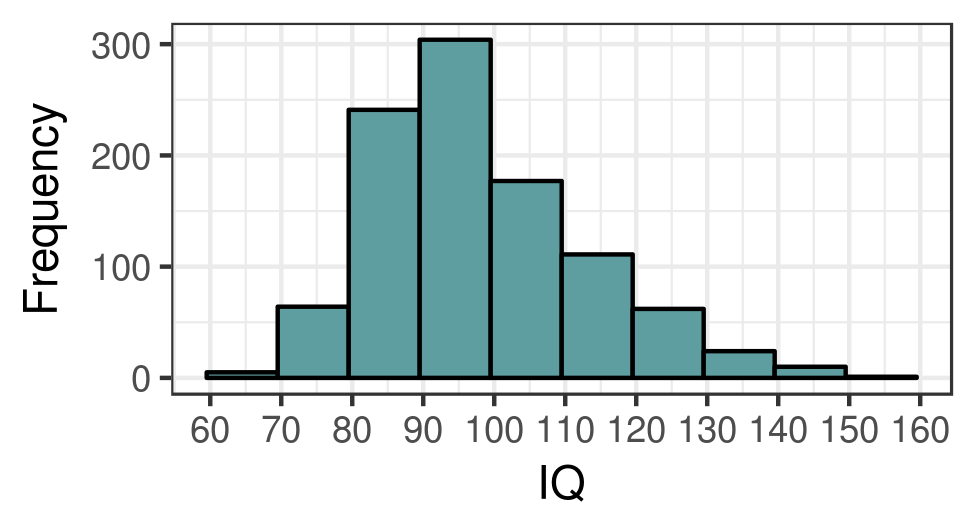
\includegraphics[width=3.25in]{../images/wk04_iq_right_hist}

\end{center}
\end{column}
\end{columns}

\end{frame}

%%%%%%%%%%
\begin{frame}{Skewed distributions, left skew example}

\begin{columns}
\begin{column}{0.35\textwidth}
\begin{exampleblock}{}
\begin{center}
\begin{tabular}{cc}
IQ & Freq \\
\hline
40 - 50 & 5 \\
50 - 60 & 16 \\
60 - 70 & 70 \\
70 - 80 & 114 \\
80 - 90 & 196 \\
90 - 100 & 293 \\
100 - 110 & 235 \\
110 - 120 & 67 \\
120 - 130 & 4 \\
\end{tabular}
\end{center}
\end{exampleblock}
\end{column}
\pause
\begin{column}{0.65\textwidth}
\begin{center}
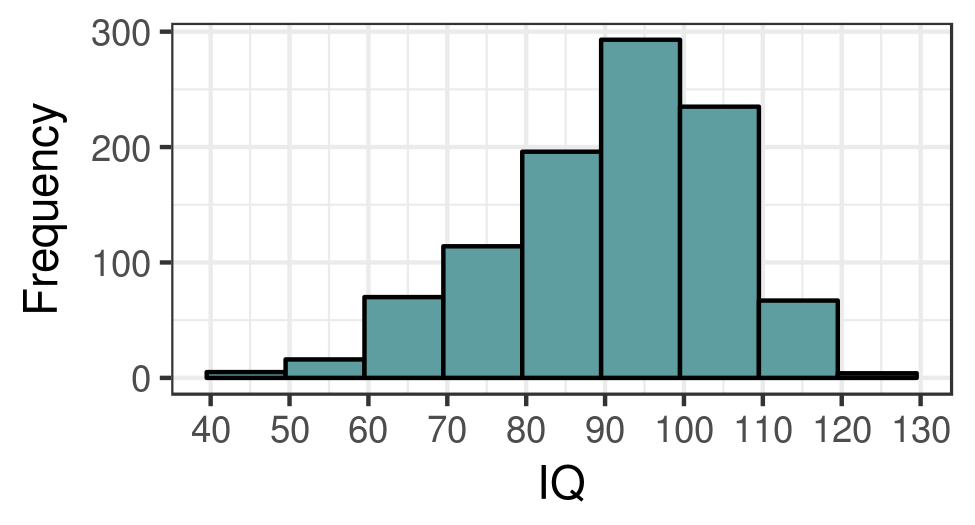
\includegraphics[width=3.25in]{../images/wk04_iq_left_hist}

\end{center}
\end{column}
\end{columns}

\end{frame}

%%%%%%%%%%
\begin{frame}
\frametitle{Bimodal distributions}
\begin{block}{}
Distributions with two peaks are known as \bt{bimodal}. They might indicate that the data come from two different populations.
\end{block}
\pause
\begin{columns}
\begin{column}{0.35\textwidth}
\begin{exampleblock}{}
\begin{center}
\begin{tabular}{cc}
Num tacos & Freq \\
\hline
0 - 1 & 1 \\
2 - 3 & 8 \\
4 - 5 & 29 \\
6 - 7 & 9 \\
8 - 9 & 3 \\
10 -11 & 3 \\
(12 - 13 & 23 \\
14 - 15 & 21 \\
16 - 17 & 3 \\
\end{tabular}
\end{center}
\end{exampleblock}
\end{column}
\pause
\begin{column}{0.65\textwidth}
\begin{center}
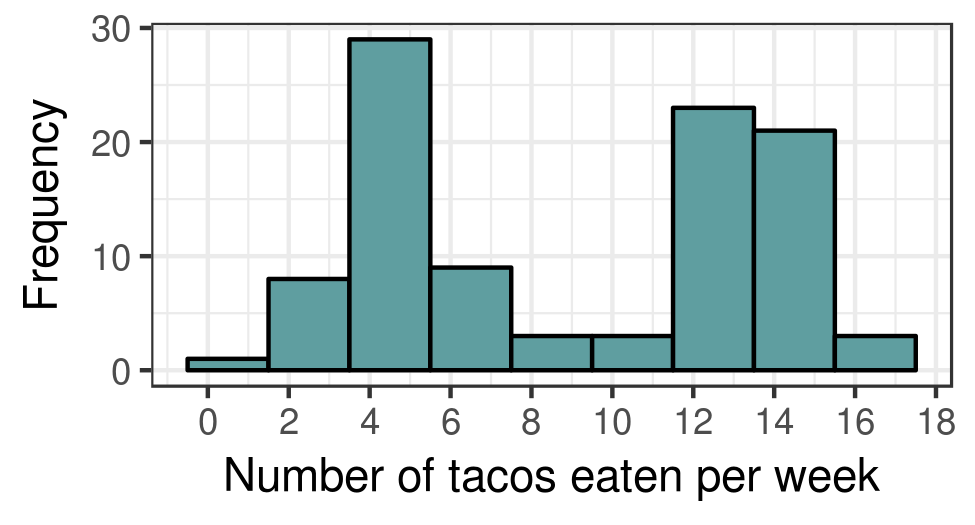
\includegraphics[width=3.25in]{../images/wk04_taco_bi_hist}

\end{center}
\end{column}
\end{columns}
\end{frame}








% 
% Section 4.2
%
\subsection{Summary Statistics}

%%%%%%%%%%
\begin{frame}
\frametitle{Measures of center}
\begin{block}{}
In order to understand a data set, values are calculated which summarize the distribution of the data or describe various properties of the data. These are, unsurprisingly, called \bt{descriptive} or \bt{summary} statistics.
\end{block}
\pause
\begin{block}{}
Perhaps the most important of these, \bt{measures of center} are a way of  representing the value of the middle of the data.\\
\medskip
There are four measures of center discussed in this section:
\begin{itemize}
\item mean
\item median
\item mode
\item midrange
\end{itemize} 
\end{block}
\end{frame}

%%%%%%%%%%
\begin{frame}{Mean}
\begin{block}{}
The \bt{mean} (the arithmetic mean) is the measure of center calculated by adding the values of the data set and dividing by the size of the data set. Also known as the average.
\begin{itemize}
\item Only makes sense with quantitative data
\item Sensitive to outliers (extreme or unusual values) and skewed data distributions.
\end{itemize}
\end{block}

\pause
\begin{block}{To calculate}
Let $X$ be sample of size $n$ of quantitative data with values $\sam x$. Then, the mean designated $\bar x$ (pronounced \bt{x bar}), is\\ \smallskip
\eq{\bar x = \frac{\sum x_i}{n}}
\begin{itemize}
\item $\sum$ means add all the $x_i$'s, where $i$ is between 1 and $n$
\end{itemize}
\end{block}
\end{frame}

%%%%%%%%%%
\begin{frame}{Mean, example}
\begin{exampleblock}{Example}
Suppose we find a sample of 8 students and ask for their ages. 

\begin{itemize}
\item The sample is $X = \set{22, 32, 46, 50, 33, 38, 20, 24}$
\pause\item The sample size is $n=8$
\pause
\item The sum of the data is\\
\smallskip
{\centering
$\sum x_i = 22 + 32 + 46 + 50 + 33 +  38 + 20 + 24 = 265$
\par}
\pause
\item The mean is\\
\smallskip
{\centering
$\ds \bar x = \frac {\sum x_i}{n} = \frac {265} 8 = 33.125 \text{ years}$
\par}
\end{itemize}
\smallskip
\end{exampleblock}
\end{frame}

%%%%%%%%%%
\begin{frame}{Median}
\begin{block}{}
The \bt{median} is the value that is greater than or equal to at least 50\% of the data and less than or equal to at least 50\% of the data.
\begin{itemize}
\item Can be used with quantitative and ordinal data (usually)
\item Not sensitive to extreme values (\bt{resistant} measure of center)
\end{itemize}
\end{block}

\pause
\begin{block}{To calculate}
Arrange the data in order, from lowest to highest.
\begin{itemize}
\item If $n$ is odd, the middle value is the median.
\item If $n$ is even, the median is the mean of the two middle values.
\end{itemize}
\end{block}
\end{frame}

%%%%%%%%%%
\begin{frame}{Median, example}
\begin{exampleblock}{Example}
Returning to the ages of 8 students.

\begin{itemize}
\item The sample is $X = \set{22, 32, 46, 50, 33, 38, 20, 24}$
\pause
\item Arranged in order, the sample looks like\\
\smallskip
{\centering
$20 \quad 22 \quad 24 \quad 32 \quad 33 \quad 38 \quad 46 \quad 50$
\par}
\pause
\item Since $n$ is even, find the the mean of the two middle values.\\
\smallskip
{\centering
$20 \quad 22 \quad 24  \underbrace{32 \quad 33}_{(32+33)/2 = 32.5}  38 \quad 46 \quad 50$
\par}
\pause
\item The median is $\tilde x = 32.5$ years.
\end{itemize}
\smallskip
\end{exampleblock}
\end{frame}

%%%%%%%%%%
\begin{frame}{Mean vs. Median}
\begin{exampleblock}{}
Suppose in our age data set, we replaced the $50$ with a $85$.
\begin{itemize}
\item Mean goes from $33.125$ to $37.5$
\item Median remains unchanged at $32.5$
\end{itemize}
\end{exampleblock}

\pause
\begin{block}{}
This is why median is called a \bt{resistant} statistic.
\begin{itemize}
\item Median is used when we don't want a few extreme values to distort a more reasonable middle, such as house prices or incomes.
\end{itemize}
\end{block}
\end{frame}

%%%%%%%%%%
\begin{frame}{Mean vs. Median, cont.}
\begin{exampleblock}{}
Suppose instead of calculating a grade point average (mean), we calculated a grade point median. Consider a student who got A's in 3 classes and D's in 2.
\begin{itemize}
\item The median grade point is 4, an A.
\item The GPA for such a student would be 2.8.
\end{itemize}
\end{exampleblock}

\pause
\begin{block}{}
The median does not consider all values of a data set. The mean does.
\begin{itemize}
\item Mean is used when all values are important or when we expect to have roughly symmetric data.
\end{itemize}
\end{block}
\end{frame}

%%%%%%%%%%
\begin{frame}{Mode}
\begin{block}{}
The \bt{mode} is the data value with highest frequency.
\begin{itemize}
\item Can be used with any kind of data.
\item A data set might have more than one mode, or there might not be any mode.
\end{itemize}
\end{block}
\end{frame}

%%%%%%%%%%
\begin{frame}{Mode, example} 
\begin{exampleblock}{Examples}
\begin{itemize}
\item The age data, $ \set{22, 32, 46, 50, 33, 38, 20, 24}$, has no mode.
\pause
\item From a TACO survey, favorite kind of taco had these responses:\\
\medskip
{\centering
$\set{\text{Beef, Beef, Fish, Shrimp, Beef, Pork, Chicken, Beef, Chicken, Beef}}$
\par}
\medskip
The mode is ``Beef'' with a frequency of five.
\pause
\item Suppose a sample from a class got the following grades on a quiz:\\
\medskip
{\centering
$\set{\text{A, C, B, A, A, B, C, B}}$
\par}
\medskip
The modes are A and B, with frequencies of three each.
\end{itemize}
\end{exampleblock}
\end{frame}

%%%%%%%%%%
\begin{frame}{Midrange}
\begin{block}{}
The \bt{midrange} is the value half way between the minimum and maximum values. Calculate by finding the mean of the minimum and maximum.
\begin{itemize}
\item Only makes sense with quantitative data.
\item \emph{Very} sensitive the extreme values.
\item Easy to calculate, but rarely used.
\end{itemize}
\end{block}

\pause
\begin{exampleblock}{Example}
The age data is $X = \set{22, 32, 46, 50, 33, 38, 20, 24}$.
\begin{itemize}
\item The minimum age is $20$ and the maximum age is $50$.
\item The midrange is \\
\smallskip
{\centering
$\ds \frac {\min(X) + \max(X)}{2} = \frac {20 + 50}{2} = 35$
\par}
\end{itemize}
\smallskip
\end{exampleblock}

\end{frame}

%%%%%%%%%%
\begin{frame}{Variation}
\begin{block}{}
Center is not the only important way to describe a distribution.
\end{block}
\pause
\bigskip
{\centering
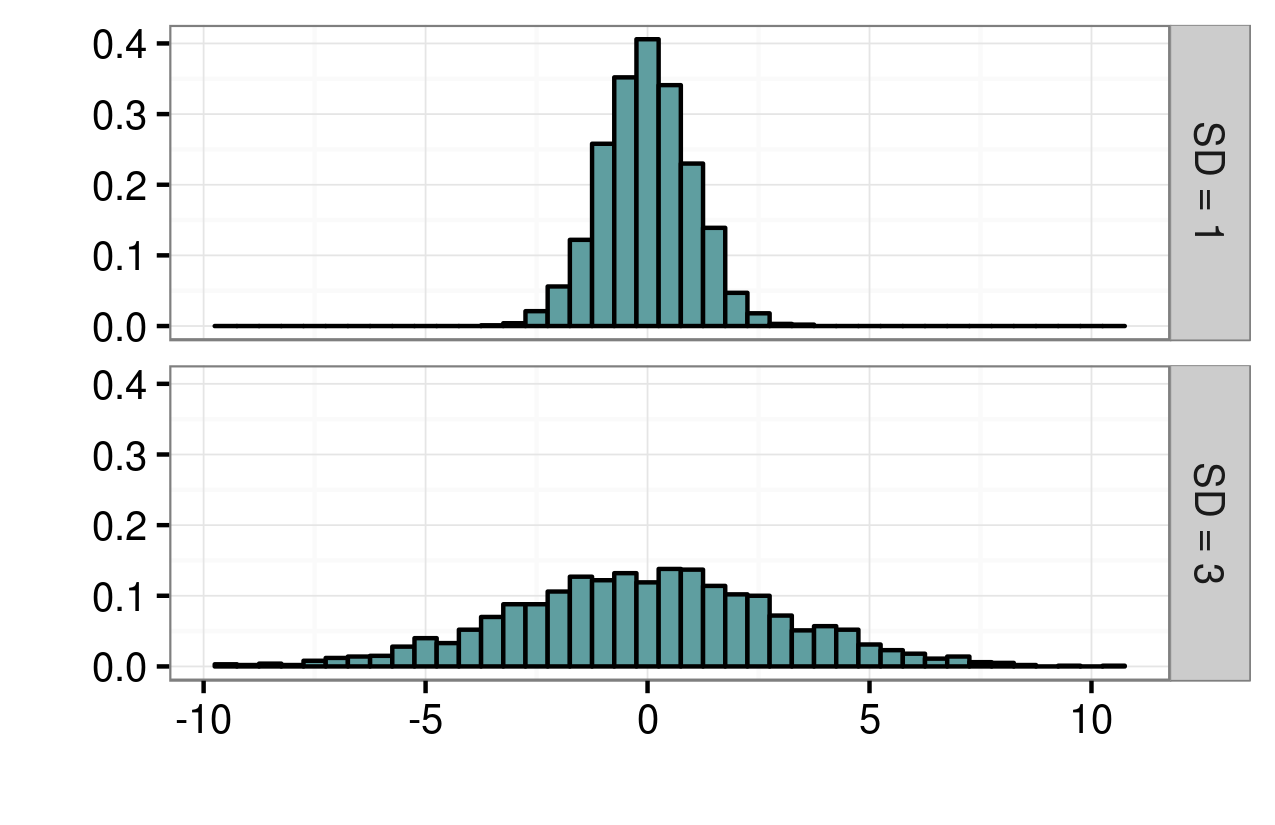
\includegraphics[width=4in]{../images/wk04_var_diff}
\par}
\end{frame}

%%%%%%%%%%
\begin{frame}{Measures of variation}
\begin{block}{}
Another important class of descriptive statistics are \bt{measures of variation} which describe how much the data is spread out.\\
\medskip
There are three measures of variation discussed in this section:
\begin{itemize}
\item Range
\item Variance
\item Standard deviation
\end{itemize}

\end{block}
\end{frame}

%%%%%%%%%%
\begin{frame}{Range}
\begin{block}{}
The \bt{range} is the difference between the maximum and minimum values.
\begin{itemize}
\item Like the midrange, very sensitive to extreme values.
\end{itemize}
\end{block}

\pause
\begin{exampleblock}{Example}
The age data is $X = \set{22, 32, 46, 50, 33, 38, 20, 24}$.
\begin{itemize}
\item The minimum age is $20$ and the maximum age is $50$.
\pause
\item The range is \\
\smallskip
{\centering
$\max(X) - \min(X) = 50 - 20 = 30 \text{ years}$
\par}
\end{itemize}
\smallskip
\end{exampleblock}

\end{frame}

%%%%%%%%%%
\begin{frame}{Variance and standard deviation}
\begin{block}{}
The \bt{variance} is the mean of the squared difference of the data from the mean. The \bt{standard deviation} is the square root of the variance.
\begin{itemize}
\pause\item More simply, the standard deviation is the average distance of the data from the data mean (the center).
\pause\item Always non-negative. A zero standard deviation means all the data are the same value.
\pause\item Sensitive to extreme values.
\pause\item The units of standard deviation are the same as the data. Variance units are the data units squared.
\end{itemize}
\end{block}
\end{frame}

%%%%%%%%%%
\begin{frame}{Variance and standard deviation, calculation}
\begin{block}{To calculate}
Let $X$ be sample of size $n$ of quantitative data with values $\sam x$ and sample mean $\bar x$. Then,\\
\smallskip
\eq{ \var(X) = s^2 = \frac{\sum (x_i - \bar x)^2}{n-1} \qquad \text{and} \qquad  \f{SD}(X) = s = \sqrt{s^2}}
\begin{itemize}
\pause\item Note: Never calculate this by hand. Use technology.
\end{itemize}
\end{block}
\end{frame}

%%%%%%%%%%
\begin{frame}{Variance and standard deviation, example}
\begin{exampleblock}{Example}
The age data is $X = \set{22, 32, 46, 50, 33, 38, 20, 24}$. The sample size is $n=8$ and the sample mean is $\bar x = 33.125$
\begin{itemize}
\pause
\item The variance is \vspace{-.1in}
\begin{align*}
s^2 &= \frac{\sum (x_i - \bar x)^2}{n-1}\\
&= \frac{(22-33.125)^2 + \cdots + (24-33.125)^2}{7}\\
&= 122.125 \text{ years}^\text{2}
\end{align*} \vspace{-.2in}
\pause\item The standard deviation is\\ \smallskip
\eq{s = \sqrt{s^2} = \sqrt{122.125} = 11.05 \text{ years}}
\end{itemize}
\smallskip
\end{exampleblock}
\end{frame}


%%%%%%%%%%
\begin{frame}{Notation}
\begin{block}{}
Recall, values that describe the properties of populations are called \bt{parameters} and values that describe samples are called \bt{statistics}. Notationally, in math formulas or when abbreviating, Greek letters are used to refer to parameters and Latin letters are used to refer to statistics.
\pause
\begin{center}
\begin{tabular}{c |r l | c}
Property & \multicolumn{2}{c|}{Parameter} & Statistic\\
\hline
Mean & $\mu$ & (mu) & $\bar x$\\
Variance & $\sigma^2$ &(sigma-squared) & $s^2$\\
Standard deviation & $\sigma$ &(sigma) & $s$
\end{tabular}
\end{center} 
\end{block}
\end{frame}


\end{document}